% =====================================================================
% main.tex
% PT: Ficheiro principal. Compile este ficheiro (pdfLaTeX + biber +
%     makeglossaries; ver README.md). Aqui só se escolhe a ordem das
%     partes do documento: os textos estão nas pastas frontmatter/,
%     chapters/ e backmatter/, e os seus dados em config/metadata.tex.
% EN: Main file. Compile this file (pdfLaTeX + biber + makeglossaries;
%     see README.md). It only sets the order of the parts of the document:
%     the texts live in frontmatter/, chapters/ and backmatter/, and your
%     data in config/metadata.tex.
% =====================================================================
\documentclass[12pt,a4paper,oneside]{report}

% PT: Pacotes e formatação, dados da dissertação e comandos próprios.
% EN: Packages and formatting, dissertation data and custom commands.
% =====================================================================
% config/packages.tex
% PT: Pacotes e formatação global (fontes, margens, espaçamento, títulos,
%     legendas, bibliografia e acrónimos). Normalmente não precisa de
%     alterar este ficheiro.
% EN: Packages and global formatting (fonts, margins, spacing, headings,
%     captions, bibliography and acronyms). You normally do not need to
%     change this file.
% =====================================================================

% ---------------------------------------------------------------------
% Codificação e idioma / Encoding and language
% ---------------------------------------------------------------------
\usepackage[T1]{fontenc}
\usepackage[utf8]{inputenc}
% PT: A última língua da lista é a língua principal do documento.
%     Para escrever a dissertação em português, troque para
%     \usepackage[english,portuguese]{babel}.
% EN: The last language in the list is the main language of the document.
%     To write the dissertation in Portuguese, change it to
%     \usepackage[english,portuguese]{babel}.
\usepackage[portuguese,english]{babel}

% ---------------------------------------------------------------------
% Fontes / Fonts
% ---------------------------------------------------------------------
% PT: O modelo ESTSetúbal/UNIPS usa Times New Roman no texto e Arial nos
%     títulos. O newtx dá a Times; se não estiver instalado, usa-se o
%     mathptmx. O helvet dá a Helvetica, com as mesmas métricas da Arial.
% EN: The ESTSetúbal/UNIPS model uses Times New Roman for body text and
%     Arial for headings. newtx provides Times; if it is not installed,
%     mathptmx is used instead. helvet provides Helvetica, which has the
%     same metrics as Arial.
% PT: O amsmath e o amsthm têm de ser carregados antes do newtxmath, e o
%     amssymb só com o mathptmx (o newtxmath já tem esses símbolos e dá
%     erro "Command \Bbbk already defined" se os dois forem carregados).
% EN: amsmath and amsthm must be loaded before newtxmath, and amssymb only
%     with mathptmx (newtxmath already has those symbols and fails with
%     "Command \Bbbk already defined" if both are loaded).
\usepackage{amsmath,amsthm}
\IfFileExists{newtxtext.sty}
  {\usepackage{newtxtext,newtxmath}}
  {\usepackage{mathptmx}\usepackage{amssymb}}
\usepackage{helvet}

% ---------------------------------------------------------------------
% Página e espaçamento / Page layout and spacing
% ---------------------------------------------------------------------
% PT: A4 com margens de 3 cm e entrelinha de 1,5.
% EN: A4 with 3 cm margins and 1.5 line spacing.
\usepackage[a4paper,margin=3cm]{geometry}
\usepackage{setspace}
\usepackage{microtype}
\usepackage{csquotes}
% PT: Indenta também o primeiro parágrafo de cada secção.
% EN: Also indent the first paragraph of each section.
\usepackage{indentfirst}

% ---------------------------------------------------------------------
% Figuras, tabelas e listas / Figures, tables and lists
% ---------------------------------------------------------------------
\usepackage{graphicx}
\usepackage{float}
\usepackage{caption}
\usepackage{subcaption}
\usepackage{booktabs}
\usepackage{tabularx}
\usepackage{longtable}
\usepackage{array}
\usepackage{multirow}
\usepackage{siunitx}
\usepackage{enumitem}
\usepackage{xcolor}
\usepackage{pdfpages}
\usepackage{etoolbox}
% PT: TikZ desenha diagramas diretamente em LaTeX (ver capítulo 3).
% EN: TikZ draws diagrams directly in LaTeX (see chapter 3).
\usepackage{tikz}
\usetikzlibrary{arrows.meta,positioning}

% ---------------------------------------------------------------------
% Matemática / Mathematics
% ---------------------------------------------------------------------
% PT: amsmath, amsthm e símbolos AMS já foram carregados com as fontes.
% EN: amsmath, amsthm and AMS symbols were already loaded with the fonts.
\usepackage{mathtools}

% ---------------------------------------------------------------------
% URLs, ligações e referências cruzadas / URLs, links and cross-references
% ---------------------------------------------------------------------
% PT: O xurl não é carregado de propósito: permite quebras após qualquer
%     carácter e parte os DOI a meio de um número. As quebras de URL na
%     bibliografia são afinadas mais abaixo.
% EN: xurl is deliberately not loaded: it allows a break after any
%     character and splits DOIs in the middle of a number. URL breaks in
%     the bibliography are tuned further below.
\PassOptionsToPackage{hyphens}{url}
\usepackage{url}
\usepackage[hidelinks]{hyperref}
\usepackage{bookmark}
% PT: \cref{...} escreve automaticamente "Figure 1.1", "Table 2.3", etc.
%     (com maiúscula, por causa da opção capitalise).
%     O cleveref não tem nomes em português europeu; em texto português
%     escreva o nome à mão: Figura~\ref{...}.
% EN: \cref{...} automatically writes "Figure 1.1", "Table 2.3", etc.
%     (capitalised, because of the capitalise option).
%     cleveref has no European Portuguese names; in Portuguese text write
%     the name by hand: Figura~\ref{...}.
\usepackage[nameinlink,noabbrev,capitalise]{cleveref}

% ---------------------------------------------------------------------
% Acrónimos / Acronyms
% ---------------------------------------------------------------------
% PT: Os acrónimos são definidos em frontmatter/acronyms.tex. A lista só
%     aparece depois de correr o makeglossaries (o latexmk fá-lo sozinho).
% EN: Acronyms are defined in frontmatter/acronyms.tex. The list only
%     appears after running makeglossaries (latexmk does it for you).
% PT: "nomain": só há lista de acrónimos, sem glossário de termos. Para
%     ter também um glossário, retire "nomain", defina os termos com
%     \newglossaryentry e junte \printglossary em main.tex.
% EN: "nomain": there is only an acronym list, no glossary of terms. To
%     also have a glossary, remove "nomain", define the terms with
%     \newglossaryentry and add \printglossary to main.tex.
\usepackage[acronym,nomain,toc]{glossaries}
\makeglossaries

% ---------------------------------------------------------------------
% Bibliografia / Bibliography
% ---------------------------------------------------------------------
% PT: Estilo IEEE (numérico, pela ordem de citação) processado pelo biber.
%     ATENÇÃO: o estilo "ieee" vem do pacote biblatex-ieee, que pode não
%     estar instalado (erro "File 'ieee.bbx' not found"). Instale-o com
%         tlmgr install biblatex-ieee
%     (MiKTeX: instale "biblatex-ieee" no MiKTeX Console) ou use a linha
%     alternativa comentada, que só precisa do biblatex.
% EN: IEEE style (numeric, in order of citation) processed by biber.
%     WARNING: the "ieee" style comes from the biblatex-ieee package, which
%     may not be installed (error "File 'ieee.bbx' not found"). Install it
%     with
%         tlmgr install biblatex-ieee
%     (MiKTeX: install "biblatex-ieee" in the MiKTeX Console) or use the
%     commented alternative line, which only needs biblatex.
\usepackage[backend=biber,style=ieee,sorting=none]{biblatex}
% \usepackage[backend=biber,style=numeric-comp,sorting=none]{biblatex}

% PT: Quebras de URL e DOI na bibliografia: só parte um número em último caso.
% EN: URL and DOI line breaks in the bibliography: break inside a number
%     only as a last resort.
\setcounter{biburllcpenalty}{7000}
\setcounter{biburlucpenalty}{8000}
\setcounter{biburlnumpenalty}{9000}
\appto{\biburlsetup}{\Urlmuskip=0mu plus 1mu\relax}
\AtBeginBibliography{\emergencystretch=4em\relax}

% ---------------------------------------------------------------------
% Espaçamento e numeração / Spacing and numbering
% ---------------------------------------------------------------------
\onehalfspacing
\setlength{\parskip}{0.4em}
\setlength{\parindent}{1.2em}

% PT: O índice mostra até às subsecções; a numeração vai até às subsubsecções.
% EN: The table of contents goes down to subsections; numbering goes down
%     to subsubsections.
\setcounter{tocdepth}{2}
\setcounter{secnumdepth}{3}

\captionsetup{font=small,labelfont=bf}

% PT: Números em formato inglês (1,234.5). Em texto português use
%     \sisetup{output-decimal-marker={,}, group-separator={\,}}
%     (ver o exemplo no capítulo 4).
% EN: Numbers in English format (1,234.5). In Portuguese text use
%     \sisetup{output-decimal-marker={,}, group-separator={\,}}
%     (see the example in chapter 4).
\sisetup{
  group-separator = {,},
  output-decimal-marker = {.}
}

% ---------------------------------------------------------------------
% Títulos (Arial/Helvetica, negrito) / Headings (Arial/Helvetica, bold)
% ---------------------------------------------------------------------
% PT: Títulos em \sffamily (Helvetica = Arial), alinhados à esquerda sem
%     hifenização, como no modelo ESTSetúbal/UNIPS.
% EN: Headings in \sffamily (Helvetica = Arial), ragged right without
%     hyphenation, as in the ESTSetúbal/UNIPS model.
\usepackage{titlesec}
\titleformat{\chapter}[display]
  {\normalfont\sffamily\huge\bfseries}
  {\chaptertitlename\ \thechapter}
  {20pt}
  {\Huge}
\titlespacing*{\chapter}{0pt}{0pt}{40pt}
\titleformat*{\section}{\normalfont\raggedright\sffamily\Large\bfseries}
\titleformat*{\subsection}{\normalfont\raggedright\sffamily\large\bfseries}
\titleformat*{\subsubsection}{\normalfont\raggedright\sffamily\normalsize\bfseries}
\titleformat*{\paragraph}{\normalfont\raggedright\sffamily\normalsize\bfseries}

% ---------------------------------------------------------------------
% Nomes das listas / Names of the lists
% ---------------------------------------------------------------------
% PT: Nomes usados quando a língua principal é o inglês.
% EN: Names used when the main language is English.
\addto\captionsenglish{%
  \renewcommand{\contentsname}{Table of Contents}%
  \renewcommand{\listfigurename}{List of Figures}%
  \renewcommand{\listtablename}{List of Tables}%
  \renewcommand{\bibname}{References}%
  \renewcommand{\refname}{References}%
}
% PT: Se a língua principal for o português, descomente estas linhas.
% EN: If the main language is Portuguese, uncomment these lines.
% \addto\captionsportuguese{%
%   \renewcommand{\contentsname}{Índice}%
%   \renewcommand{\listfigurename}{Índice de Figuras}%
%   \renewcommand{\listtablename}{Índice de Tabelas}%
%   \renewcommand{\bibname}{Referências Bibliográficas}%
%   \renewcommand{\refname}{Referências Bibliográficas}%
% }

% =====================================================================
% config/metadata.tex
% PT: Dados da dissertação. É aqui que preenche o título, o seu nome, o
%     curso, os orientadores, o júri e as datas. A capa, a folha do júri e
%     as propriedades do PDF são geradas a partir destes valores.
%     Substitua apenas o texto entre as chavetas finais { }.
% EN: Dissertation data. This is where you fill in the title, your name,
%     the programme, the supervisors, the jury and the dates. The cover,
%     the jury page and the PDF properties are generated from these values.
%     Replace only the text inside the last pair of braces { }.
% =====================================================================

% ---------------------------------------------------------------------
% Trabalho / Work
% ---------------------------------------------------------------------
% PT: Título da dissertação. Na capa é escrito em maiúsculas.
%     Ex.: Deteção de Anomalias em Redes Industriais com Aprendizagem Automática
% EN: Dissertation title. It is printed in capitals on the cover.
%     E.g.: Anomaly Detection in Industrial Networks with Machine Learning
\newcommand{\thesistitle}{Título da Dissertação}

% PT: Subtítulo opcional. Se não estiver vazio, aparece na capa e na folha
%     do júri a seguir ao título, separado por dois pontos. Deixe {} vazio
%     se não tiver subtítulo.
%     Ex.: Um Estudo de Caso no Setor Automóvel
% EN: Optional subtitle. If not empty, it is printed on the cover and the
%     jury page after the title, separated by a colon. Leave {} empty if
%     there is no subtitle.
%     E.g.: A Case Study in the Automotive Sector
\newcommand{\thesissubtitle}{}

% PT: Palavras-chave para as propriedades do PDF (separadas por vírgulas).
%     As palavras-chave visíveis estão em abstract.tex e resumo.tex.
%     Ex.: Machine Learning, Anomaly Detection, Industrial Networks
% EN: Keywords for the PDF properties (comma-separated). The visible
%     keywords are in abstract.tex and resumo.tex.
%     E.g.: Machine Learning, Anomaly Detection, Industrial Networks
\newcommand{\thesiskeywords}{Palavra-chave 1, Palavra-chave 2, Palavra-chave 3}

% ---------------------------------------------------------------------
% Aluno e curso / Student and programme
% ---------------------------------------------------------------------
% PT: Nome completo do aluno, como deve aparecer na capa (em maiúsculas).
%     Ex.: Ana Exemplo Ferreira
% EN: Student's full name, as it should appear on the cover (in capitals).
%     E.g.: Ana Exemplo Ferreira
\newcommand{\authorname}{Nome Completo do Aluno}

% PT: Nome completo do mestrado (usado nas propriedades do PDF).
%     Ex.: Mestrado em Engenharia de Software
% EN: Full name of the master's programme (used in the PDF properties).
%     E.g.: Mestrado em Engenharia de Software
\newcommand{\coursename}{Mestrado em Nome do Curso}

% PT: Primeira linha do bloco do grau na capa. Use o tipo de trabalho que
%     se aplica ao seu caso (Dissertação, Projeto ou Estágio).
%     Ex.: Relatório de Dissertação do Mestrado em
% EN: First line of the degree block on the cover. Use the type of work
%     that applies to you (Dissertação, Projeto or Estágio).
%     E.g.: Relatório de Dissertação do Mestrado em
\newcommand{\coverdegree}{Relatório de Dissertação do Mestrado em}

% PT: Segunda linha do bloco do grau na capa: a área do mestrado.
%     Ex.: Engenharia de Software
% EN: Second line of the degree block on the cover: the programme field.
%     E.g.: Engenharia de Software
\newcommand{\coursefield}{Nome do Curso}

% PT: Instituição e escola (usadas nas propriedades do PDF).
% EN: University and school (used in the PDF properties).
\newcommand{\institutionname}{Universidade Politécnica de Setúbal}
\newcommand{\schoolname}{Escola Superior de Tecnologia de Setúbal}

% PT: Cidade (disponível para uso no texto, ex.: nos agradecimentos).
% EN: City (available for use in the text, e.g. in the acknowledgements).
\newcommand{\cityname}{Setúbal}

% ---------------------------------------------------------------------
% Orientação / Supervision
% ---------------------------------------------------------------------
% PT: Orientador, com grau académico.
%     Ex.: Prof. Doutor João Exemplo Almeida
% EN: Supervisor, with academic title.
%     E.g.: Prof. Doutor João Exemplo Almeida
\newcommand{\supervisorname}{Prof. Doutor Nome do Orientador}

% PT: Coorientador (OPCIONAL). Se deixar {} vazio, a capa não mostra o
%     bloco COORIENTADOR.
%     Ex.: Prof.ª Doutora Maria Exemplo Sousa   ou   {} (sem coorientador)
% EN: Co-supervisor (OPTIONAL). If you leave {} empty, the cover does not
%     show the COORIENTADOR block.
%     E.g.: Prof.ª Doutora Maria Exemplo Sousa   or   {} (no co-supervisor)
\newcommand{\cosupervisorname}{Prof. Doutor Nome do Coorientador}

% PT: Rótulos da capa e da folha do júri. Mude para a forma feminina
%     (ORIENTADORA, COORIENTADORA, Orientadora) quando se aplicar.
% EN: Labels on the cover and the jury page. Change them to the feminine
%     form (ORIENTADORA, COORIENTADORA, Orientadora) when it applies.
\newcommand{\supervisorlabel}{ORIENTADOR}
\newcommand{\cosupervisorlabel}{COORIENTADOR}
\newcommand{\juryadvisorlabel}{Orientador}

% ---------------------------------------------------------------------
% Datas / Dates
% ---------------------------------------------------------------------
% PT: Mês (em minúsculas, em português) e ano de entrega.
%     Ex.: novembro  /  2026
% EN: Month (lowercase, in Portuguese) and year of submission.
%     E.g.: novembro  /  2026
\newcommand{\submissionmonth}{mês}
\newcommand{\submissionyear}{AAAA}

% PT: Mês e ano da prova pública (defesa). Aparecem no fundo da capa e da
%     folha do júri. Por omissão são iguais aos da entrega; depois da
%     defesa, substitua por valores concretos.
%     Ex.: \newcommand{\defencemonth}{janeiro}  /  \newcommand{\defenceyear}{2027}
% EN: Month and year of the public defence. They are printed at the bottom
%     of the cover and the jury page. By default they match the submission
%     date; after the defence, replace them with the actual values.
%     E.g.: \newcommand{\defencemonth}{janeiro}  /  \newcommand{\defenceyear}{2027}
\newcommand{\defencemonth}{\submissionmonth}
\newcommand{\defenceyear}{\submissionyear}

% ---------------------------------------------------------------------
% Júri (folha do júri) / Jury (jury page)
% ---------------------------------------------------------------------
% PT: Formato de cada membro: Grau Nome, Instituição.
% EN: Format of each member: Title Name, Institution.

% PT: Presidente do júri.
%     Ex.: Prof. Doutor Rui Exemplo Lopes, Universidade Politécnica de Setúbal
% EN: Jury president.
%     E.g.: Prof. Doutor Rui Exemplo Lopes, Universidade Politécnica de Setúbal
\newcommand{\jurypresident}{Prof. Doutor Nome do Presidente, Universidade Politécnica de Setúbal}

% PT: Orientador no júri (normalmente igual a \supervisorname + instituição).
% EN: Supervisor on the jury (usually \supervisorname + institution).
\newcommand{\juryadvisor}{Prof. Doutor Nome do Orientador, Universidade Politécnica de Setúbal}

% PT: Vogal (arguente). É obrigatório pelo menos um.
%     Ex.: Prof.ª Doutora Carla Exemplo Pinto, Universidade de Lisboa
% EN: Examiner ("vogal"). At least one is required.
%     E.g.: Prof.ª Doutora Carla Exemplo Pinto, Universidade de Lisboa
\newcommand{\juryvogal}{Prof. Doutor Nome do Vogal, Instituição}

% PT: Segundo vogal (OPCIONAL). Deixe {} vazio se o júri tiver só um
%     vogal; preencha-o se tiver dois. Cada vogal ocupa uma linha.
%     Ex.: Prof. Doutor Tiago Exemplo Nunes, Universidade de Évora
% EN: Second examiner (OPTIONAL). Leave {} empty if the jury has a single
%     examiner; fill it in if there are two. Each examiner takes one line.
%     E.g.: Prof. Doutor Tiago Exemplo Nunes, Universidade de Évora
\newcommand{\jurysecondvogal}{}

% =====================================================================
% config/commands.tex
% PT: Comandos auxiliares próprios. Acrescente aqui os seus comandos
%     (\newcommand) para os manter num só sítio.
% EN: Helper commands of your own. Add your commands (\newcommand) here
%     to keep them in one place.
% =====================================================================

% PT: Caixa vazia para marcar uma figura que ainda não existe.
%     Uso: \placeholderfigure{<largura>}{<altura>}
%     Ex.: \placeholderfigure{0.8\textwidth}{5cm}
% EN: Empty box to mark a figure that does not exist yet.
%     Usage: \placeholderfigure{<width>}{<height>}
%     E.g.: \placeholderfigure{0.8\textwidth}{5cm}
\newcommand{\placeholderfigure}[2]{%
  \begin{center}
    \fbox{\parbox[c][#2][c]{#1}{\centering Figure placeholder / Figura provisória\\[0.5em]
    Replace with the final image. / Substituir pela imagem final.}}
  \end{center}
}

% PT: Nota de trabalho a azul, para lembretes durante a escrita.
%     Apague todas antes da entrega. Uso: \todosection{texto}
% EN: Work note in blue, for reminders while writing.
%     Remove them all before submission. Usage: \todosection{text}
\newcommand{\todosection}[1]{%
  \begin{quote}
    \color{blue!70!black}\textbf{TODO:} #1
  \end{quote}
}

% PT: Questões de investigação e objetivos numerados.
%     Uso: \researchq{1}{Texto da questão}  ->  RQ1. Texto da questão
% EN: Numbered research questions and objectives.
%     Usage: \researchq{1}{Question text}  ->  RQ1. Question text
\newcommand{\researchq}[2]{\textbf{RQ#1.} #2}
\newcommand{\researchobj}[2]{\textbf{OBJ#1.} #2}

% PT: Coluna Y para tabularx: ocupa a largura disponível e alinha à esquerda.
%     Uso: \begin{tabularx}{\textwidth}{lY} ... \end{tabularx}
% EN: Y column for tabularx: fills the available width, left-aligned.
%     Usage: \begin{tabularx}{\textwidth}{lY} ... \end{tabularx}
\newcolumntype{Y}{>{\raggedright\arraybackslash}X}


% PT: Propriedades do PDF, preenchidas a partir de config/metadata.tex.
% EN: PDF properties, filled in from config/metadata.tex.
\hypersetup{
  pdftitle={\thesistitle},
  pdfauthor={\authorname},
  pdfsubject={\coursename\ -- \schoolname, \institutionname},
  pdfkeywords={\thesiskeywords}
}

% PT: Lista de acrónimos e ficheiro da bibliografia.
% EN: Acronym list and bibliography file.
% =====================================================================
% frontmatter/acronyms.tex
% PT: Lista de siglas e acrónimos. Cada sigla é definida uma vez aqui e
%     usada no texto com \gls{rótulo}. A lista é ordenada automaticamente.
% EN: List of acronyms. Each acronym is defined once here and used in the
%     text with \gls{label}. The list is sorted automatically.
%
% PT: Formato: \newacronym{rótulo}{SIGLA}{Forma por extenso}
%     No texto:
%       \gls{ai}       1.º uso: "Artificial Intelligence (AI)"; depois: "AI"
%       \glspl{cnn}    plural: "Convolutional Neural Networks (CNNs)" / "CNNs"
%       \Gls{ai}       com maiúscula inicial, no início de uma frase
%       \acrshort{ai}  só a sigla: "AI"
%       \acrlong{ai}   só a forma por extenso: "Artificial Intelligence"
%       \acrfull{ai}   sempre completa: "Artificial Intelligence (AI)"
% EN: Format: \newacronym{label}{ACRONYM}{Long form}
%     In the text:
%       \gls{ai}       1st use: "Artificial Intelligence (AI)"; then: "AI"
%       \glspl{cnn}    plural: "Convolutional Neural Networks (CNNs)" / "CNNs"
%       \Gls{ai}       capitalised, at the start of a sentence
%       \acrshort{ai}  acronym only: "AI"
%       \acrlong{ai}   long form only: "Artificial Intelligence"
%       \acrfull{ai}   always full: "Artificial Intelligence (AI)"
% =====================================================================

% PT: Exemplos em inglês.
% EN: English examples.
\newacronym{ai}{AI}{Artificial Intelligence}
\newacronym{ml}{ML}{Machine Learning}
\newacronym{cnn}{CNN}{Convolutional Neural Network}

% PT: Exemplo de sigla portuguesa, para texto escrito em português.
% EN: Example of a Portuguese acronym, for text written in Portuguese.
\newacronym{ia}{IA}{Inteligência Artificial}

\addbibresource{bibliography/references.bib}

\begin{document}

% ---------------------------------------------------------------------
% PT: Capa e folha do júri (sem número de página).
% EN: Cover and jury page (no page number).
% ---------------------------------------------------------------------
\pagenumbering{gobble}
% =====================================================================
% frontmatter/cover.tex
% PT: Capa (página 1 do modelo ESTSetúbal/UNIPS). Reproduz a primeira
%     página de TrabalhoUNIPS_TecnologiaSetubal_Mestrado_definitiva.docx.
%     NÃO precisa de editar este ficheiro: o texto vem de
%     config/metadata.tex. NÃO altere as posições \put nem as medidas em
%     bp, porque copiam o modelo oficial do Word.
% EN: Cover (page 1 of the ESTSetúbal/UNIPS model). Reproduces the first
%     page of TrabalhoUNIPS_TecnologiaSetubal_Mestrado_definitiva.docx.
%     You do NOT need to edit this file: the text comes from
%     config/metadata.tex. Do NOT change the \put positions or the bp
%     measurements, because they copy the official Word model.
%
% PT: Como funciona
%     - Página A4 = 595 x 842 bp (1 bp = 1 ponto do Word = 1/72 pol.).
%     - Cada bloco é colocado com \put(x,-y) em relação ao canto superior
%       esquerdo da página: x para a direita, y para baixo (daí o sinal -).
%     - Fonte Arial (Helvetica, com as mesmas métricas), sem hifenização.
%     - No Word, cada caixa de texto tem margem interna de 7.2 bp à
%       esquerda e 3.6 bp no topo; por isso cada \put fica em
%       x = caixa + 7.2 e y = topo da caixa + 3.6 + ascendente da Arial,
%       ou seja, na linha de base da primeira linha do bloco.
% EN: How it works
%     - A4 page = 595 x 842 bp (1 bp = 1 Word point = 1/72 in).
%     - Each block is placed with \put(x,-y) relative to the top-left
%       corner of the page: x to the right, y downwards (hence the - sign).
%     - Arial font (Helvetica, with the same metrics), no hyphenation.
%     - In Word each text box has an inner margin of 7.2 bp on the left and
%       3.6 bp at the top; so each \put sits at x = box + 7.2 and
%       y = box top + 3.6 + Arial ascender, i.e. on the baseline of the
%       first line of the block.
%
% PT: Medidas das caixas do Word (bp, a partir do canto superior esquerdo)
% EN: Word text-box measurements (bp, from the top-left corner)
%   logotipo / logo        x = 191.05, topo/top y = 67, largura/width 255.4
%   autor / author         x = 85.15,  y = 263.4, largura/width 160.0, 16 pt, à direita/right-aligned
%   título / title         x = 249.95, y = 263.0, largura/width 290.1, 16 pt negrito/bold
%   grau / degree          x = 249.95, y = 460.0, largura/width 275.1, 12 pt
%   linha / line           centro/centre x = 250.65, y = 263.5 -> 773.7, 3.75 pt, #CAF4FF
%   orientadores / supervisors  x = 250.25, y = 582.2, largura/width 275.1, 12 pt
%   data / date            x = 250.25, y = 735.5, 10 pt
%
% PT: Título longo
%     O título (16 pt, entrelinha 18.4 bp) começa na linha de base
%     y = 278.6 e o bloco do grau começa em y = 472.0. Cabem no máximo
%     10 linhas de título (cerca de 20 a 28 caracteres em maiúsculas por
%     linha, ou seja, uns 220 caracteres no total); a 11.ª linha sobrepõe-se
%     ao bloco do grau. Para um aspeto equilibrado, mantenha o título até
%     8 linhas. O subtítulo conta para estas linhas. Se não couber,
%     encurte o título; pode também forçar as quebras de linha com \\ no
%     próprio \thesistitle. A folha do júri aceita até 12 linhas, por isso
%     o limite é dado pela capa.
% EN: Long title
%     The title (16 pt, 18.4 bp leading) starts on baseline y = 278.6 and
%     the degree block starts at y = 472.0. At most 10 title lines fit
%     (roughly 20 to 28 capital letters per line, about 220 characters in
%     total); an 11th line overlaps the degree block. For a balanced look,
%     keep the title within 8 lines. The subtitle counts towards these
%     lines. If it does not fit, shorten the title; you can also force
%     line breaks with \\ inside \thesistitle. The jury page accepts up to
%     12 lines, so the cover sets the limit.
% =====================================================================
\begin{titlepage}
% PT: Os blocos são desenhados por cima da página, no momento em que ela é
%     enviada para o PDF, com coordenadas absolutas.
% EN: The blocks are drawn on top of the page, when it is shipped out to
%     the PDF, with absolute coordinates.
\AddToHookNext{shipout/foreground}{%
  \setlength{\unitlength}{1bp}%
  \linespread{1}\fontfamily{phv}\fontseries{m}\fontshape{n}\selectfont
  \hyphenpenalty=10000 \exhyphenpenalty=10000
  % -------------------------------------------------------------------
  % PT: Logotipo da ESTSetúbal/UNIPS (figures/estsetubal_logo.pdf), centrado no topo.
  % EN: ESTSetúbal/UNIPS logo (figures/estsetubal_logo.pdf), centred at the top.
  \put(191.05,-67){\makebox(0,0)[lt]{
\includegraphics[width=255.4bp]{figures/estsetubal_logo.pdf}}}%
  % -------------------------------------------------------------------
  % PT: Autor: coluna da esquerda, 16 pt regular, maiúsculas, alinhado à direita.
  % EN: Author: left column, 16 pt regular, capitals, right-aligned.
  \put(92.35,-279.0){\parbox[t]{145.6bp}{\raggedleft\fontsize{16bp}{18.4bp}\selectfont
    \MakeUppercase{\authorname}}}%
  % -------------------------------------------------------------------
  % PT: Título (e subtítulo opcional): coluna da direita, 16 pt negrito, maiúsculas.
  % EN: Title (and optional subtitle): right column, 16 pt bold, capitals.
  \put(257.15,-278.6){\parbox[t]{275.7bp}{\raggedright\fontsize{16bp}{18.4bp}\selectfont\bfseries
    \MakeUppercase{\thesistitle}\ifdefempty{\thesissubtitle}{}{\MakeUppercase{: \thesissubtitle}}}}%
  % -------------------------------------------------------------------
  % PT: Grau: duas linhas, 12 pt regular (\coverdegree e \coursefield).
  % EN: Degree: two lines, 12 pt regular (\coverdegree and \coursefield).
  \put(257.15,-472.0){\parbox[t]{260.7bp}{\raggedright\fontsize{12bp}{13.8bp}\selectfont
    \coverdegree\par\coursefield}}%
  % -------------------------------------------------------------------
  % PT: Linha azul vertical #CAF4FF entre as duas colunas (no Word é uma
  %     linha de 510.2 pt rodada 270 graus).
  % EN: Vertical blue line #CAF4FF between the two columns (in Word it is a
  %     510.2 pt line rotated 270 degrees).
  \put(248.775,-773.7){\textcolor[HTML]{CAF4FF}{\rule{3.75bp}{510.2bp}}}%
  % -------------------------------------------------------------------
  % PT: Orientador e coorientador, 12 pt. O bloco COORIENTADOR só aparece
  %     se \cosupervisorname não estiver vazio.
  % EN: Supervisor and co-supervisor, 12 pt. The COORIENTADOR block only
  %     appears if \cosupervisorname is not empty.
  \put(257.45,-594.2){\parbox[t]{260.7bp}{\raggedright\fontsize{12bp}{13.8bp}\selectfont
    \setlength{\parskip}{2bp}\setlength{\parindent}{0pt}%
    {\bfseries \supervisorlabel\par}
    \supervisorname\par
    \ifdefempty{\cosupervisorname}{}{%
      \vspace{6bp}
      {\bfseries \cosupervisorlabel\par}
      \cosupervisorname\par}}}%
  % -------------------------------------------------------------------
  % PT: Data da realização da prova (mês e ano), 10 pt.
  % EN: Date of the public defence (month and year), 10 pt.
  \put(257.45,-747.4){\parbox[t]{230.5bp}{\raggedright\fontsize{10bp}{13.2bp}\selectfont
    \defencemonth\ de \defenceyear}}%
}
% PT: Página vazia: o conteúdo é todo desenhado pelo bloco acima.
% EN: Empty page: all content is drawn by the block above.
\null
\end{titlepage}

\clearpage
% =====================================================================
% frontmatter/folha-rosto.tex
% PT: Folha do júri (página 2 do modelo ESTSetúbal/UNIPS). Reproduz a
%     segunda página de TrabalhoUNIPS_TecnologiaSetubal_Mestrado_definitiva.docx.
%     NÃO precisa de editar este ficheiro: o texto vem de
%     config/metadata.tex. NÃO altere as posições \put nem as medidas em
%     bp. O sistema de coordenadas está explicado em frontmatter/cover.tex.
% EN: Jury page (page 2 of the ESTSetúbal/UNIPS model). Reproduces the
%     second page of TrabalhoUNIPS_TecnologiaSetubal_Mestrado_definitiva.docx.
%     You do NOT need to edit this file: the text comes from
%     config/metadata.tex. Do NOT change the \put positions or the bp
%     measurements. The coordinate system is explained in
%     frontmatter/cover.tex.
%
% PT: Medidas das caixas do Word (bp, a partir do canto superior esquerdo)
% EN: Word text-box measurements (bp, from the top-left corner)
%   autor / author   x = 85.05,  y = 263.4, largura/width 160.0, 16 pt, à direita/right-aligned
%   título / title   x = 249.95, y = 263.0, largura/width 290.1, 16 pt negrito/bold
%   linha / line     centro/centre x = 249.95, y = 263.5 -> 773.7, 3.75 pt, #CAF4FF
%   júri / jury      x = 249.95, y = 501.0, largura/width 275.1, 11 pt, entrelinha/leading 1.15
%   data / date      x = 250.15, y = 735.5, 10 pt
%
% PT: Nesta página o título pode ter até 12 linhas (a 13.ª encosta ao
%     bloco do júri, em y = 514.0); o limite prático é o da capa (10
%     linhas, ver frontmatter/cover.tex).
% EN: On this page the title can take up to 12 lines (a 13th line touches
%     the jury block, at y = 514.0); the practical limit is the cover's
%     (10 lines, see frontmatter/cover.tex).
% =====================================================================
\begin{titlepage}
\AddToHookNext{shipout/foreground}{%
  \setlength{\unitlength}{1bp}%
  \linespread{1}\fontfamily{phv}\fontseries{m}\fontshape{n}\selectfont
  \hyphenpenalty=10000 \exhyphenpenalty=10000
  % -------------------------------------------------------------------
  % PT: Autor: coluna da esquerda, 16 pt regular, maiúsculas, alinhado à direita.
  % EN: Author: left column, 16 pt regular, capitals, right-aligned.
  \put(92.25,-279.0){\parbox[t]{145.6bp}{\raggedleft\fontsize{16bp}{18.4bp}\selectfont
    \MakeUppercase{\authorname}}}%
  % -------------------------------------------------------------------
  % PT: Título (e subtítulo opcional): coluna da direita, 16 pt negrito, maiúsculas.
  % EN: Title (and optional subtitle): right column, 16 pt bold, capitals.
  \put(257.15,-278.6){\parbox[t]{275.7bp}{\raggedright\fontsize{16bp}{18.4bp}\selectfont\bfseries
    \MakeUppercase{\thesistitle}\ifdefempty{\thesissubtitle}{}{\MakeUppercase{: \thesissubtitle}}}}%
  % -------------------------------------------------------------------
  % PT: Linha azul vertical #CAF4FF (no Word: linha de 510.2 pt rodada 270 graus).
  % EN: Vertical blue line #CAF4FF (in Word: 510.2 pt line rotated 270 degrees).
  \put(248.075,-773.7){\textcolor[HTML]{CAF4FF}{\rule{3.75bp}{510.2bp}}}%
  % -------------------------------------------------------------------
  % PT: Júri, 11 pt, entrelinha 1,15. Uma linha por membro: Presidente,
  %     Orientador e um ou dois vogais. A linha do segundo vogal só aparece
  %     se \jurysecondvogal não estiver vazio (ver config/metadata.tex).
  % EN: Jury, 11 pt, 1.15 line spacing. One line per member: president,
  %     supervisor and one or two examiners ("vogais"). The second
  %     examiner's line only appears if \jurysecondvogal is not empty
  %     (see config/metadata.tex).
  \put(257.15,-514.0){\parbox[t]{260.7bp}{\raggedright\fontsize{11bp}{14.55bp}\selectfont
    \setlength{\parindent}{0pt}\setlength{\parskip}{0pt}%
    {\bfseries JÚRI\par}
    \mbox{}\par
    Presidente: \jurypresident\par
    \juryadvisorlabel: \juryadvisor\par
    Vogal: \juryvogal\par
    \ifdefempty{\jurysecondvogal}{}{Vogal: \jurysecondvogal\par}}}%
  % -------------------------------------------------------------------
  % PT: Data da realização da prova (mês e ano), 10 pt.
  % EN: Date of the public defence (month and year), 10 pt.
  \put(257.35,-747.4){\parbox[t]{230.5bp}{\raggedright\fontsize{10bp}{13.2bp}\selectfont
    \defencemonth\ de \defenceyear}}%
}
% PT: Página vazia: o conteúdo é todo desenhado pelo bloco acima.
% EN: Empty page: all content is drawn by the block above.
\null
\end{titlepage}

\clearpage

% ---------------------------------------------------------------------
% PT: Elementos pré-textuais, numerados em romano (i, ii, iii, ...).
% EN: Front matter, numbered in Roman numerals (i, ii, iii, ...).
% ---------------------------------------------------------------------
\pagenumbering{roman}
\setcounter{page}{1}

% =====================================================================
% frontmatter/acknowledgements.tex
% PT: Agradecimentos. Capítulo sem número que aparece no índice.
%     É opcional: se não o quiser, apague a linha
%     % =====================================================================
% frontmatter/acknowledgements.tex
% PT: Agradecimentos. Capítulo sem número que aparece no índice.
%     É opcional: se não o quiser, apague a linha
%     % =====================================================================
% frontmatter/acknowledgements.tex
% PT: Agradecimentos. Capítulo sem número que aparece no índice.
%     É opcional: se não o quiser, apague a linha
%     \input{frontmatter/acknowledgements} em main.tex.
% EN: Acknowledgements. Unnumbered chapter listed in the table of
%     contents. It is optional: if you do not want it, delete the line
%     \input{frontmatter/acknowledgements} in main.tex.
% =====================================================================

% PT: Numa dissertação em português, use \chapter*{Agradecimentos} e
%     \addcontentsline{toc}{chapter}{Agradecimentos}.
% EN: In a dissertation written in Portuguese, use
%     \chapter*{Agradecimentos} and \addcontentsline{toc}{chapter}{Agradecimentos}.
\chapter*{Acknowledgements}
\addcontentsline{toc}{chapter}{Acknowledgements}

% PT: Exemplo em inglês.
% EN: English example.
\noindent\textbf{English example.}
I would like to thank my supervisor, \supervisorname, for the guidance and
availability throughout this work. I also thank my family and friends for
their support during the master's programme.

\bigskip

% PT: Exemplo em português.
% EN: Portuguese example.
\begin{otherlanguage}{portuguese}
\noindent\textbf{Exemplo em português.}
Agradeço ao meu orientador, \supervisorname, pela orientação e pela
disponibilidade ao longo deste trabalho. Agradeço também à minha família e
aos meus amigos pelo apoio durante o mestrado.
\end{otherlanguage}

% PT: Assinatura opcional no fim da página.
% EN: Optional signature at the bottom of the page.
% \vfill
% \begin{flushright}
%   \authorname\\
%   \cityname, \submissionmonth\ de \submissionyear
% \end{flushright}
 em main.tex.
% EN: Acknowledgements. Unnumbered chapter listed in the table of
%     contents. It is optional: if you do not want it, delete the line
%     % =====================================================================
% frontmatter/acknowledgements.tex
% PT: Agradecimentos. Capítulo sem número que aparece no índice.
%     É opcional: se não o quiser, apague a linha
%     \input{frontmatter/acknowledgements} em main.tex.
% EN: Acknowledgements. Unnumbered chapter listed in the table of
%     contents. It is optional: if you do not want it, delete the line
%     \input{frontmatter/acknowledgements} in main.tex.
% =====================================================================

% PT: Numa dissertação em português, use \chapter*{Agradecimentos} e
%     \addcontentsline{toc}{chapter}{Agradecimentos}.
% EN: In a dissertation written in Portuguese, use
%     \chapter*{Agradecimentos} and \addcontentsline{toc}{chapter}{Agradecimentos}.
\chapter*{Acknowledgements}
\addcontentsline{toc}{chapter}{Acknowledgements}

% PT: Exemplo em inglês.
% EN: English example.
\noindent\textbf{English example.}
I would like to thank my supervisor, \supervisorname, for the guidance and
availability throughout this work. I also thank my family and friends for
their support during the master's programme.

\bigskip

% PT: Exemplo em português.
% EN: Portuguese example.
\begin{otherlanguage}{portuguese}
\noindent\textbf{Exemplo em português.}
Agradeço ao meu orientador, \supervisorname, pela orientação e pela
disponibilidade ao longo deste trabalho. Agradeço também à minha família e
aos meus amigos pelo apoio durante o mestrado.
\end{otherlanguage}

% PT: Assinatura opcional no fim da página.
% EN: Optional signature at the bottom of the page.
% \vfill
% \begin{flushright}
%   \authorname\\
%   \cityname, \submissionmonth\ de \submissionyear
% \end{flushright}
 in main.tex.
% =====================================================================

% PT: Numa dissertação em português, use \chapter*{Agradecimentos} e
%     \addcontentsline{toc}{chapter}{Agradecimentos}.
% EN: In a dissertation written in Portuguese, use
%     \chapter*{Agradecimentos} and \addcontentsline{toc}{chapter}{Agradecimentos}.
\chapter*{Acknowledgements}
\addcontentsline{toc}{chapter}{Acknowledgements}

% PT: Exemplo em inglês.
% EN: English example.
\noindent\textbf{English example.}
I would like to thank my supervisor, \supervisorname, for the guidance and
availability throughout this work. I also thank my family and friends for
their support during the master's programme.

\bigskip

% PT: Exemplo em português.
% EN: Portuguese example.
\begin{otherlanguage}{portuguese}
\noindent\textbf{Exemplo em português.}
Agradeço ao meu orientador, \supervisorname, pela orientação e pela
disponibilidade ao longo deste trabalho. Agradeço também à minha família e
aos meus amigos pelo apoio durante o mestrado.
\end{otherlanguage}

% PT: Assinatura opcional no fim da página.
% EN: Optional signature at the bottom of the page.
% \vfill
% \begin{flushright}
%   \authorname\\
%   \cityname, \submissionmonth\ de \submissionyear
% \end{flushright}
 em main.tex.
% EN: Acknowledgements. Unnumbered chapter listed in the table of
%     contents. It is optional: if you do not want it, delete the line
%     % =====================================================================
% frontmatter/acknowledgements.tex
% PT: Agradecimentos. Capítulo sem número que aparece no índice.
%     É opcional: se não o quiser, apague a linha
%     % =====================================================================
% frontmatter/acknowledgements.tex
% PT: Agradecimentos. Capítulo sem número que aparece no índice.
%     É opcional: se não o quiser, apague a linha
%     \input{frontmatter/acknowledgements} em main.tex.
% EN: Acknowledgements. Unnumbered chapter listed in the table of
%     contents. It is optional: if you do not want it, delete the line
%     \input{frontmatter/acknowledgements} in main.tex.
% =====================================================================

% PT: Numa dissertação em português, use \chapter*{Agradecimentos} e
%     \addcontentsline{toc}{chapter}{Agradecimentos}.
% EN: In a dissertation written in Portuguese, use
%     \chapter*{Agradecimentos} and \addcontentsline{toc}{chapter}{Agradecimentos}.
\chapter*{Acknowledgements}
\addcontentsline{toc}{chapter}{Acknowledgements}

% PT: Exemplo em inglês.
% EN: English example.
\noindent\textbf{English example.}
I would like to thank my supervisor, \supervisorname, for the guidance and
availability throughout this work. I also thank my family and friends for
their support during the master's programme.

\bigskip

% PT: Exemplo em português.
% EN: Portuguese example.
\begin{otherlanguage}{portuguese}
\noindent\textbf{Exemplo em português.}
Agradeço ao meu orientador, \supervisorname, pela orientação e pela
disponibilidade ao longo deste trabalho. Agradeço também à minha família e
aos meus amigos pelo apoio durante o mestrado.
\end{otherlanguage}

% PT: Assinatura opcional no fim da página.
% EN: Optional signature at the bottom of the page.
% \vfill
% \begin{flushright}
%   \authorname\\
%   \cityname, \submissionmonth\ de \submissionyear
% \end{flushright}
 em main.tex.
% EN: Acknowledgements. Unnumbered chapter listed in the table of
%     contents. It is optional: if you do not want it, delete the line
%     % =====================================================================
% frontmatter/acknowledgements.tex
% PT: Agradecimentos. Capítulo sem número que aparece no índice.
%     É opcional: se não o quiser, apague a linha
%     \input{frontmatter/acknowledgements} em main.tex.
% EN: Acknowledgements. Unnumbered chapter listed in the table of
%     contents. It is optional: if you do not want it, delete the line
%     \input{frontmatter/acknowledgements} in main.tex.
% =====================================================================

% PT: Numa dissertação em português, use \chapter*{Agradecimentos} e
%     \addcontentsline{toc}{chapter}{Agradecimentos}.
% EN: In a dissertation written in Portuguese, use
%     \chapter*{Agradecimentos} and \addcontentsline{toc}{chapter}{Agradecimentos}.
\chapter*{Acknowledgements}
\addcontentsline{toc}{chapter}{Acknowledgements}

% PT: Exemplo em inglês.
% EN: English example.
\noindent\textbf{English example.}
I would like to thank my supervisor, \supervisorname, for the guidance and
availability throughout this work. I also thank my family and friends for
their support during the master's programme.

\bigskip

% PT: Exemplo em português.
% EN: Portuguese example.
\begin{otherlanguage}{portuguese}
\noindent\textbf{Exemplo em português.}
Agradeço ao meu orientador, \supervisorname, pela orientação e pela
disponibilidade ao longo deste trabalho. Agradeço também à minha família e
aos meus amigos pelo apoio durante o mestrado.
\end{otherlanguage}

% PT: Assinatura opcional no fim da página.
% EN: Optional signature at the bottom of the page.
% \vfill
% \begin{flushright}
%   \authorname\\
%   \cityname, \submissionmonth\ de \submissionyear
% \end{flushright}
 in main.tex.
% =====================================================================

% PT: Numa dissertação em português, use \chapter*{Agradecimentos} e
%     \addcontentsline{toc}{chapter}{Agradecimentos}.
% EN: In a dissertation written in Portuguese, use
%     \chapter*{Agradecimentos} and \addcontentsline{toc}{chapter}{Agradecimentos}.
\chapter*{Acknowledgements}
\addcontentsline{toc}{chapter}{Acknowledgements}

% PT: Exemplo em inglês.
% EN: English example.
\noindent\textbf{English example.}
I would like to thank my supervisor, \supervisorname, for the guidance and
availability throughout this work. I also thank my family and friends for
their support during the master's programme.

\bigskip

% PT: Exemplo em português.
% EN: Portuguese example.
\begin{otherlanguage}{portuguese}
\noindent\textbf{Exemplo em português.}
Agradeço ao meu orientador, \supervisorname, pela orientação e pela
disponibilidade ao longo deste trabalho. Agradeço também à minha família e
aos meus amigos pelo apoio durante o mestrado.
\end{otherlanguage}

% PT: Assinatura opcional no fim da página.
% EN: Optional signature at the bottom of the page.
% \vfill
% \begin{flushright}
%   \authorname\\
%   \cityname, \submissionmonth\ de \submissionyear
% \end{flushright}
 in main.tex.
% =====================================================================

% PT: Numa dissertação em português, use \chapter*{Agradecimentos} e
%     \addcontentsline{toc}{chapter}{Agradecimentos}.
% EN: In a dissertation written in Portuguese, use
%     \chapter*{Agradecimentos} and \addcontentsline{toc}{chapter}{Agradecimentos}.
\chapter*{Acknowledgements}
\addcontentsline{toc}{chapter}{Acknowledgements}

% PT: Exemplo em inglês.
% EN: English example.
\noindent\textbf{English example.}
I would like to thank my supervisor, \supervisorname, for the guidance and
availability throughout this work. I also thank my family and friends for
their support during the master's programme.

\bigskip

% PT: Exemplo em português.
% EN: Portuguese example.
\begin{otherlanguage}{portuguese}
\noindent\textbf{Exemplo em português.}
Agradeço ao meu orientador, \supervisorname, pela orientação e pela
disponibilidade ao longo deste trabalho. Agradeço também à minha família e
aos meus amigos pelo apoio durante o mestrado.
\end{otherlanguage}

% PT: Assinatura opcional no fim da página.
% EN: Optional signature at the bottom of the page.
% \vfill
% \begin{flushright}
%   \authorname\\
%   \cityname, \submissionmonth\ de \submissionyear
% \end{flushright}

\clearpage
% =====================================================================
% frontmatter/abstract.tex
% PT: Resumo em inglês (Abstract). Um único parágrafo, normalmente com
%     150 a 300 palavras (confirme o limite no regulamento em vigor).
%     Deve dizer: contexto, problema, abordagem, principais resultados e
%     conclusão. As palavras-chave (normalmente 3 a 6) vão no fim, na linha
%     "Keywords", separadas por ponto e vírgula.
% EN: Abstract in English. A single paragraph, usually 150 to 300 words
%     (check the limit in the current regulations). It should state:
%     context, problem, approach, main results and conclusion. The keywords
%     (usually 3 to 6) go at the end, on the "Keywords" line, separated by
%     semicolons.
% =====================================================================
\chapter*{Abstract}
\addcontentsline{toc}{chapter}{Abstract}

% PT: Texto de exemplo em inglês: substitua pelo seu resumo.
% EN: Example text in English: replace it with your abstract.
This is an example abstract. In a real dissertation, this paragraph
summarises the whole work for a reader who will not read anything else. It
starts with one or two sentences of context that explain why the topic
matters, then states the problem or gap the dissertation addresses. Next, it
describes the approach in concrete terms: the method, the data or case
study, and the tools that were used. It then reports the main results,
preferably with the key numbers, and closes with the main conclusion and
what it means for practice or for future research. The abstract should not
contain citations, figures, tables or undefined acronyms, and every claim in
it should be supported by the main text. Write it last, once the results and
conclusions are final, and keep it within the word limit set by the school.

\vspace{1em}
% PT: Palavras-chave em inglês (3 a 6), separadas por ponto e vírgula.
% EN: Keywords in English (3 to 6), separated by semicolons.
\noindent\textbf{Keywords:} Keyword One; Keyword Two; Keyword Three; Keyword Four

\clearpage
% =====================================================================
% frontmatter/resumo.tex
% PT: Resumo em português europeu. Tradução fiel do Abstract, também num
%     único parágrafo com 150 a 300 palavras (confirme o limite no
%     regulamento em vigor). As palavras-chave (normalmente 3 a 6) vão no
%     fim, na linha "Palavras-chave", separadas por ponto e vírgula, pela
%     mesma ordem das Keywords.
% EN: Abstract in European Portuguese. A faithful translation of the
%     Abstract, also a single paragraph of 150 to 300 words (check the
%     limit in the current regulations). The keywords (usually 3 to 6) go
%     at the end, on the "Palavras-chave" line, separated by semicolons, in
%     the same order as the English keywords.
% =====================================================================

% PT: O ambiente otherlanguage aplica a hifenização portuguesa.
% EN: The otherlanguage environment applies Portuguese hyphenation.
\begin{otherlanguage}{portuguese}
\chapter*{Resumo}
\addcontentsline{toc}{chapter}{Resumo}

% PT: Texto de exemplo em português europeu: substitua pelo seu resumo.
% EN: Example text in European Portuguese: replace it with your abstract.
Este é um resumo de exemplo. Numa dissertação real, este parágrafo
sintetiza todo o trabalho para um leitor que não vai ler mais nada. Começa
com uma ou duas frases de contexto que explicam a relevância do tema e
indica depois o problema ou a lacuna a que a dissertação dá resposta. Em
seguida, descreve a abordagem em termos concretos: o método, os dados ou o
caso de estudo e as ferramentas utilizadas. Apresenta depois os principais
resultados, de preferência com os valores mais importantes, e termina com a
conclusão principal e o seu significado para a prática ou para investigação
futura. O resumo não deve conter citações, figuras, tabelas nem siglas por
definir, e todas as afirmações devem estar fundamentadas no texto
principal. Escreva-o no fim, quando os resultados e as conclusões estiverem
fechados, e respeite o limite de palavras definido pela escola.

\vspace{1em}
% PT: Palavras-chave em português (3 a 6), separadas por ponto e vírgula.
% EN: Keywords in Portuguese (3 to 6), separated by semicolons.
\noindent\textbf{Palavras-chave:} Palavra-chave Um; Palavra-chave Dois; Palavra-chave Três; Palavra-chave Quatro
\end{otherlanguage}

\clearpage
\selectlanguage{english}

% PT: Numa dissertação em português, traduza os títulos desta secção e da
%     bibliografia (ex.: "Índice", "Lista de Figuras", "Lista de Tabelas",
%     "Lista de Siglas e Acrónimos", "Referências Bibliográficas").
% EN: In a dissertation written in Portuguese, translate the titles in this
%     section and in the bibliography (see the examples above).
\pdfbookmark[0]{Table of Contents}{toc}
\tableofcontents
\clearpage

\addcontentsline{toc}{chapter}{List of Figures}
\listoffigures
\clearpage

\addcontentsline{toc}{chapter}{List of Tables}
\listoftables

% PT: Mostra todos os acrónimos definidos, mesmo os que ainda não foram
%     usados no texto. Para mostrar só os usados, apague \glsaddallunused.
% EN: Lists every defined acronym, even those not used in the text yet.
%     To list only the ones used, delete \glsaddallunused.
\glsaddallunused
\printglossary[type=\acronymtype, title={List of Acronyms}, toctitle={List of Acronyms}, nonumberlist]
\clearpage

% ---------------------------------------------------------------------
% PT: Corpo do texto, numerado em árabe (1, 2, 3, ...). Para acrescentar
%     um capítulo, crie chapters/07-nome.tex e junte aqui \input{...}.
% EN: Main text, numbered in Arabic numerals (1, 2, 3, ...). To add a
%     chapter, create chapters/07-name.tex and add \input{...} here.
% ---------------------------------------------------------------------
\pagenumbering{arabic}
\setcounter{page}{1}
% PT: O primeiro uso de cada acrónimo no corpo do texto volta a ser por
%     extenso, mesmo que já tenha aparecido no resumo.
% EN: The first use of each acronym in the main text is spelled out again,
%     even if it already appeared in the abstract.
\glsresetall

% =====================================================================
% chapters/01-introduction.tex
% PT: Capítulo 1 -- Introdução. Exemplo de: parágrafo de abertura,
%     secções e subsecções, acrónimos (\gls), citação (\cite), nota de
%     rodapé, listas itemize/enumerate e referências cruzadas a capítulos
%     e secções (\cref, \ref).
% EN: Chapter 1 -- Introduction. Shows: opening paragraph, sections and
%     subsections, acronyms (\gls), citation (\cite), footnote,
%     itemize/enumerate lists and cross-references to chapters and
%     sections (\cref, \ref).
% =====================================================================

% PT: Cada capítulo tem um \label para poder ser referido noutros sítios.
%     Prefixos sugeridos: chap: capítulo, sec: secção, fig: figura,
%     tab: tabela, eq: equação, app: apêndice.
% EN: Each chapter has a \label so it can be referred to elsewhere.
%     Suggested prefixes: chap: chapter, sec: section, fig: figure,
%     tab: table, eq: equation, app: appendix.
\chapter{Introduction}
\label{chap:introduction}

% PT: Parágrafo de abertura: em poucas frases, diz ao leitor o que o
%     capítulo contém, antes da primeira secção.
% EN: Opening paragraph: in a few sentences, tell the reader what the
%     chapter contains, before the first section.
This chapter shows how a chapter is written with this template. In a real
dissertation, the introduction presents the context of the work, the problem
it addresses, its objectives and research questions, and the structure of the
document. Every chapter of the template contains a short English example
followed by a Portuguese example; together they cover the features you are
most likely to need. Replace the text and keep the structure.

% ---------------------------------------------------------------------
% PT: Exemplo em inglês
% EN: English example
% ---------------------------------------------------------------------
\section{English example}
\label{sec:intro:en}

\subsection{Context and Motivation}
\label{sec:intro:context}

% PT: \gls escreve a sigla por extenso no primeiro uso e abreviada depois.
% EN: \gls spells out the acronym on first use and abbreviates it afterwards.
Research in \gls{ai}, and in particular in \gls{ml}, has changed the way
data are analysed in many fields \cite{LeCun2015}. From the second use
onwards, only the short form is printed: \gls{ai} and \gls{ml}.
% PT: Nota de rodapé: o texto vai dentro de \footnote{...}.
% EN: Footnote: the text goes inside \footnote{...}.
The context section should explain why the topic matters and who benefits
from the work.\footnote{Footnotes are numbered per chapter. Use them sparingly,
for side remarks that would interrupt the main text.}

\subsection{Objectives}
\label{sec:intro:objectives}

The general objective of a dissertation is usually stated in one sentence and
then broken down into specific objectives:

% PT: Lista com marcas (itemize).
% EN: Bulleted list (itemize).
\begin{itemize}
  \item review the state of the art on the topic;
  \item design and implement the proposed solution;
  \item evaluate the solution against a baseline;
  \item discuss the results and their limitations.
\end{itemize}

\subsection{Research Questions}
\label{sec:intro:questions}

% PT: Lista numerada (enumerate). O enumitem permite rótulos próprios.
% EN: Numbered list (enumerate). enumitem allows custom labels.
\begin{enumerate}[label=\textbf{RQ\arabic*.}, leftmargin=*]
  \item Which methods are currently used to solve the problem?
  \item How does the proposed solution compare with those methods?
  \item Under which conditions does the proposed solution fail?
\end{enumerate}

\subsection{Document Structure}
\label{sec:intro:structure}

% PT: \cref escreve o tipo e o número ("Chapter 2"). \Cref é a forma
%     para o início da frase; com a opção capitalise, usada neste
%     template, as duas dão o mesmo resultado em inglês.
% EN: \cref writes the type and the number ("Chapter 2"). \Cref is the
%     form for the start of a sentence; with the capitalise option, used in
%     this template, both give the same result in English.
\Cref{chap:review} reviews the related work. \Cref{chap:methodology}
describes the methodology and \cref{chap:results} reports the results, which
are discussed in \cref{chap:discussion}. \Cref{chap:conclusion} concludes the
document, and \cref{app:example} holds supporting material. The objectives
listed in \cref{sec:intro:objectives} are revisited in the conclusion.

% ---------------------------------------------------------------------
% PT: Exemplo em português
% EN: Portuguese example
% ---------------------------------------------------------------------
\section{Exemplo em português}
\label{sec:intro:pt}

% PT: O ambiente otherlanguage aplica a hifenização portuguesa ao bloco.
% EN: The otherlanguage environment applies Portuguese hyphenation to the block.
\begin{otherlanguage}{portuguese}

\subsection{Enquadramento}

% PT: Sigla portuguesa definida em frontmatter/acronyms.tex.
% EN: Portuguese acronym defined in frontmatter/acronyms.tex.
A \gls{ia} tem vindo a ser aplicada em áreas tão diferentes como a
indústria, a saúde e a educação \cite{Goodfellow2016}. Depois do primeiro
uso, a sigla aparece só abreviada: \gls{ia}. O enquadramento deve explicar
a relevância do tema e o problema concreto que a dissertação
resolve.\footnote{As notas de rodapé funcionam da mesma forma em texto
português.}

\subsection{Objetivos}

% PT: Em texto português, escreva o nome à mão antes de \ref.
% EN: In Portuguese text, write the name by hand before \ref.
Os objetivos específicos seguem a ordem dos capítulos, descrita na
Secção~\ref{sec:intro:structure}:

\begin{enumerate}
  \item rever o estado da arte (Capítulo~\ref{chap:review});
  \item conceber e implementar a solução (Capítulo~\ref{chap:methodology});
  \item avaliar e discutir os resultados (Capítulos~\ref{chap:results}
        e~\ref{chap:discussion}).
\end{enumerate}

\end{otherlanguage}

% =====================================================================
% chapters/02-literature-review.tex
% PT: Capítulo 2 -- Revisão da literatura. Exemplo de: citações com
%     \cite e \textcite, várias fontes numa citação, citação com página,
%     fonte online e acrónimos no plural (\glspl).
% EN: Chapter 2 -- Literature review. Shows: citations with \cite and
%     \textcite, several sources in one citation, citation with a page
%     number, an online source and plural acronyms (\glspl).
% =====================================================================
\chapter{Literature Review}
\label{chap:review}

% PT: Parágrafo de abertura do capítulo.
% EN: Chapter opening paragraph.
This chapter shows how to cite sources. In a real dissertation, the
literature review presents the concepts the work builds on, summarises and
compares the related work, and ends by identifying the gap the dissertation
fills. Every source cited here must have an entry in
\texttt{bibliography/references.bib}; the reference list at the end of the
document is generated automatically and only contains the sources that are
cited.

% ---------------------------------------------------------------------
% PT: Exemplo em inglês
% EN: English example
% ---------------------------------------------------------------------
\section{English example}
\label{sec:review:en}

\subsection{Citing Sources}
\label{sec:review:citing}

% PT: \cite{chave} dá "[1]"; \textcite{chave} dá "Autor et al. [1]".
%     A chave é o identificador da entrada no ficheiro .bib.
% EN: \cite{key} gives "[1]"; \textcite{key} gives "Author et al. [1]".
%     The key is the identifier of the entry in the .bib file.
Deep learning methods learn representations of data with several levels of
abstraction \cite{LeCun2015}. \textcite{Goodfellow2016} give a comprehensive
introduction to the field, and \textcite{He2016} showed that residual
connections make it possible to train much deeper \glspl{cnn}.

% PT: Várias fontes de uma vez e citação de uma página concreta.
% EN: Several sources at once and citation of a specific page.
Several sources can be cited together \cite{LeCun2015,He2016}, and a
specific page can be added in square brackets \cite[p.~164]{Goodfellow2016}.
Online sources, such as software documentation, are cited in the same way
\cite{CTANbiblatexieee}.

\subsection{Summary of Related Work}
\label{sec:review:summary}

A literature review should do more than list papers. Group the works by
approach, compare them on the criteria that matter for your problem, and
close the chapter by stating clearly what is still missing. A comparison
table, like the one in \cref{tab:results}, is often a good way to summarise
the related work.

% ---------------------------------------------------------------------
% PT: Exemplo em português
% EN: Portuguese example
% ---------------------------------------------------------------------
\section{Exemplo em português}
\label{sec:review:pt}

\begin{otherlanguage}{portuguese}

Os métodos de aprendizagem profunda aprendem representações dos dados com
vários níveis de abstração \cite{LeCun2015}. Segundo
\textcite{Goodfellow2016}, estas representações são aprendidas diretamente a
partir dos dados, sem regras definidas à mão. \textcite{He2016} mostraram que
as ligações residuais permitem treinar \glspl{cnn} com muito mais camadas.

Para acrescentar uma nova fonte, crie uma entrada no ficheiro
\texttt{references.bib} com uma chave única (por exemplo,
\texttt{Silva2024}) e cite-a no texto com \texttt{\textbackslash
cite\{Silva2024\}}.

\end{otherlanguage}

% =====================================================================
% chapters/03-methodology.tex
% PT: Capítulo 3 -- Metodologia. Exemplo de: figura desenhada com TikZ
%     (sem ficheiro de imagem), equação numerada, números e unidades com
%     siunitx e referências a figura, equação e secção.
% EN: Chapter 3 -- Methodology. Shows: a figure drawn with TikZ (no image
%     file needed), a numbered equation, numbers and units with siunitx,
%     and references to a figure, an equation and a section.
% =====================================================================
\chapter{Methodology}
\label{chap:methodology}

% PT: Parágrafo de abertura do capítulo.
% EN: Chapter opening paragraph.
This chapter shows how to include a diagram and an equation. In a real
dissertation, the methodology describes what was done and how, in enough
detail for someone else to repeat the work: the overall approach, the data,
the methods and the experimental setup.

% ---------------------------------------------------------------------
% PT: Exemplo em inglês
% EN: English example
% ---------------------------------------------------------------------
\section{English example}
\label{sec:method:en}

\subsection{Overview}
\label{sec:method:overview}

% PT: Figura TikZ. [htbp] deixa o LaTeX escolher o melhor sítio:
%     h = aqui, t = topo, b = fundo, p = página própria.
%     Não use \gls dentro de \caption (use \acrshort), porque a legenda
%     também é escrita na lista de figuras.
% EN: TikZ figure. [htbp] lets LaTeX choose the best place:
%     h = here, t = top, b = bottom, p = separate page.
%     Do not use \gls inside \caption (use \acrshort), because the caption
%     is also written to the list of figures.
\begin{figure}[htbp]
  \centering
  \begin{tikzpicture}[
      node distance=8mm,
      stage/.style={draw, rounded corners, fill=blue!8, align=center,
                    minimum height=12mm, text width=24mm, font=\small\sffamily},
      arrow/.style={-{Stealth[length=2.5mm]}, thick}
    ]
    \node[stage] (data) {Data\\collection};
    \node[stage, right=of data] (prep) {Pre-\\processing};
    \node[stage, right=of prep] (model) {Model\\training};
    \node[stage, right=of model] (eval) {Evaluation};
    \draw[arrow] (data) -- (prep);
    \draw[arrow] (prep) -- (model);
    \draw[arrow] (model) -- (eval);
    \draw[arrow, dashed] (eval.south) -- ++(0,-8mm)
      -| node[pos=0.25, below, font=\footnotesize\sffamily] {adjust and repeat}
      (model.south);
  \end{tikzpicture}
  \caption{Example of a methodology diagram drawn with TikZ: the stages of a
    generic \acrshort{ml} pipeline.}
  \label{fig:pipeline}
\end{figure}

% PT: \cref{fig:...} escreve "Figure 3.1" com ligação.
% EN: \cref{fig:...} writes "Figure 3.1" with a link.
\Cref{fig:pipeline} summarises the methodology. Data are collected and
pre-processed, a model is trained, and the model is evaluated; the dashed
arrow shows that training is repeated with new settings until the
evaluation criteria are met. Diagrams drawn with TikZ use the same fonts as
the text and scale without loss of quality.

\subsection{Model}
\label{sec:method:model}

% PT: Equação numerada: o número aparece à direita, por capítulo (3.1).
%     Refira-a com \cref{eq:...} ou \eqref{eq:...}.
% EN: Numbered equation: the number appears on the right, per chapter
%     (3.1). Refer to it with \cref{eq:...} or \eqref{eq:...}.
A \gls{cnn} classifier is trained by minimising the cross-entropy loss over
the $N$ training examples and $C$ classes, given in \cref{eq:loss}:
\begin{equation}
  \mathcal{L}(\theta) = -\frac{1}{N} \sum_{i=1}^{N} \sum_{c=1}^{C}
  y_{i,c} \log \hat{y}_{i,c}(\theta),
  \label{eq:loss}
\end{equation}
where $\theta$ are the model parameters, $y_{i,c}$ is $1$ if example $i$
belongs to class $c$ and $0$ otherwise, and $\hat{y}_{i,c}(\theta)$ is the
probability predicted by the model.

\subsection{Experimental Setup}
\label{sec:method:setup}

% PT: siunitx: \num{...} para números e \qty{número}{unidade} para
%     quantidades (o antigo \SI{...}{...} continua a funcionar).
% EN: siunitx: \num{...} for numbers and \qty{number}{unit} for quantities
%     (the older \SI{...}{...} still works).
The model was trained on \num{50000} images for \num{30} epochs, with a
learning rate of \num{1e-3} and a batch size of \num{64}. The experiments ran
on a workstation with a \qty{3.2}{\giga\hertz} processor, \qty{32}{\giga\byte}
of memory and a graphics card with \qty{12}{\giga\byte} of memory. The setup
must allow the evaluation in \cref{sec:results:en} to be reproduced.

% ---------------------------------------------------------------------
% PT: Exemplo em português
% EN: Portuguese example
% ---------------------------------------------------------------------
\section{Exemplo em português}
\label{sec:method:pt}

\begin{otherlanguage}{portuguese}

% PT: Referências em português: nome à mão + \ref; \eqref põe parênteses.
% EN: References in Portuguese: name by hand + \ref; \eqref adds parentheses.
A Figura~\ref{fig:pipeline} resume as etapas da metodologia, descritas na
Secção~\ref{sec:method:overview}. O modelo é treinado minimizando a função
de perda da Equação~\eqref{eq:loss}. Na metodologia, descreva o que foi feito
com detalhe suficiente para que outra pessoa possa repetir o trabalho:
dados, métodos, ferramentas e parâmetros.

\end{otherlanguage}

% =====================================================================
% chapters/04-results.tex
% PT: Capítulo 4 -- Resultados. Exemplo de: tabela com booktabs e colunas
%     numéricas alinhadas (siunitx), figura a partir de um ficheiro em
%     figures/, e números no formato português (vírgula decimal).
% EN: Chapter 4 -- Results. Shows: a table with booktabs and aligned
%     numeric columns (siunitx), a figure from a file in figures/, and
%     numbers in Portuguese format (decimal comma).
% =====================================================================
\chapter{Results}
\label{chap:results}

% PT: Parágrafo de abertura do capítulo.
% EN: Chapter opening paragraph.
This chapter shows how to present results in a table and in a figure. In a
real dissertation, the results chapter reports what was measured, in the
order of the research questions, and leaves the interpretation for the
discussion. All values in this chapter are illustrative.

% ---------------------------------------------------------------------
% PT: Exemplo em inglês
% EN: English example
% ---------------------------------------------------------------------
\section{English example}
\label{sec:results:en}

\subsection{Results Table}
\label{sec:results:table}

% PT: Tabela com booktabs: use só \toprule, \midrule e \bottomrule, sem
%     linhas verticais. A legenda das tabelas vai por cima.
%     Colunas S (siunitx) alinham os números pela vírgula/ponto decimal;
%     table-format=2.1 significa 2 algarismos inteiros e 1 decimal.
%     Cabeçalhos de colunas S vão entre chavetas { }.
% EN: Table with booktabs: use only \toprule, \midrule and \bottomrule,
%     with no vertical lines. Table captions go above the table.
%     S columns (siunitx) align numbers on the decimal marker;
%     table-format=2.1 means 2 integer digits and 1 decimal.
%     Headers of S columns go inside braces { }.
\begin{table}[htbp]
  \centering
  \caption{Example of a results table with booktabs and siunitx
    (illustrative values).}
  \label{tab:results}
  \begin{tabular}{l S[table-format=2.1] S[table-format=1.3] S[table-format=2.1]}
    \toprule
    {Method} & {Accuracy (\%)} & {F1-score} & {Training time (min)} \\
    \midrule
    Baseline          & 78.4 & 0.762 & 12.5 \\
    Method A          & 84.1 & 0.829 & 18.0 \\
    Method B          & 86.7 & 0.851 & 25.3 \\
    Proposed method   & 89.2 & 0.884 & 21.7 \\
    \bottomrule
  \end{tabular}
\end{table}

% PT: Números e unidades no texto: \num, \qty e \percent.
% EN: Numbers and units in the text: \num, \qty and \percent.
\Cref{tab:results} compares the proposed method with a baseline and two
alternatives. The proposed method reaches an accuracy of \qty{89.2}{\percent}
and an F1-score of \num{0.884}, while taking \qty{21.7}{\minute} to train.
Bold or colour can highlight the best value, but the table should be
readable without them.

\subsection{Results Figure}
\label{sec:results:figure}

% PT: Figura a partir de um ficheiro. Prefira PDF (vetorial) para gráficos
%     e PNG/JPG para fotografias. A legenda das figuras vai por baixo.
% EN: Figure from a file. Prefer PDF (vector) for charts and PNG/JPG for
%     photographs. Figure captions go below the figure.
\begin{figure}[htbp]
  \centering
  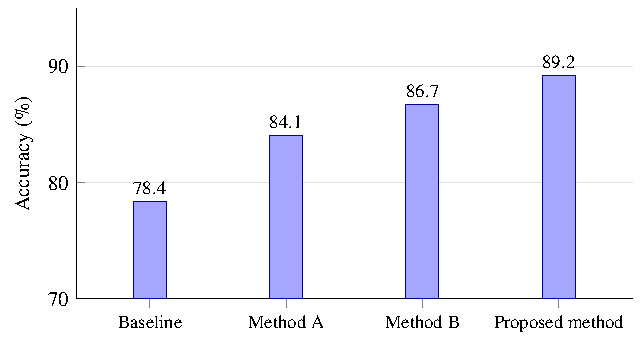
\includegraphics[width=0.75\textwidth]{figures/example-figure.pdf}
  \caption{Example of a figure included from a PDF file: accuracy of each
    method in \cref{tab:results} (illustrative values).}
  \label{fig:example-file}
\end{figure}

\Cref{fig:example-file} shows the same accuracy values as a chart. Charts
are easier to compare at a glance, while tables give the exact values; use
the one that best supports the point you are making.

% ---------------------------------------------------------------------
% PT: Exemplo em português
% EN: Portuguese example
% ---------------------------------------------------------------------
\section{Exemplo em português}
\label{sec:results:pt}

\begin{otherlanguage}{portuguese}
% PT: Formato português dos números só dentro deste bloco: vírgula decimal
%     e espaço fino a separar os milhares.
% EN: Portuguese number format only inside this block: decimal comma and a
%     thin space as thousands separator.
\sisetup{output-decimal-marker={,}, group-separator={\,}}

A Tabela~\ref{tab:results} e a Figura~\ref{fig:example-file} apresentam os
resultados. O método proposto atinge uma exatidão de
\qty{89.2}{\percent} e um F1-score de \num{0.884}, com um tempo de treino de
\qty{21.7}{\minute}, num conjunto de \num{50000} imagens. No ficheiro
\texttt{.tex}, os números escrevem-se sempre com ponto decimal; o siunitx
encarrega-se de os mostrar com vírgula.

\end{otherlanguage}

% =====================================================================
% chapters/05-discussion.tex
% PT: Capítulo 5 -- Discussão. Exemplo de: referências cruzadas entre
%     capítulos (várias de uma vez), variantes dos acrónimos (\acrshort,
%     \acrlong, \acrfull), lista itemize e nota de rodapé.
% EN: Chapter 5 -- Discussion. Shows: cross-references between chapters
%     (several at once), acronym variants (\acrshort, \acrlong, \acrfull),
%     an itemize list and a footnote.
% =====================================================================
\chapter{Discussion}
\label{chap:discussion}

% PT: Parágrafo de abertura do capítulo.
% EN: Chapter opening paragraph.
This chapter shows how to refer back to earlier material. In a real
dissertation, the discussion interprets the results, relates them to the
literature, answers the research questions and states the limitations of the
work.

% ---------------------------------------------------------------------
% PT: Exemplo em inglês
% EN: English example
% ---------------------------------------------------------------------
\section{English example}
\label{sec:discussion:en}

\subsection{Interpretation of the Results}
\label{sec:discussion:interpretation}

% PT: \cref aceita várias etiquetas separadas por vírgulas e agrupa-as:
%     \cref{fig:a,fig:b} -> "Figures 3.1 and 4.1".
% EN: \cref accepts several labels separated by commas and groups them:
%     \cref{fig:a,fig:b} -> "Figures 3.1 and 4.1".
The results in \cref{tab:results} follow the pipeline of \cref{fig:pipeline},
and \cref{fig:pipeline,fig:example-file} can be cited together. The loss in
\cref{eq:loss} was the only training objective, as described in
\cref{sec:method:model}. These references stay correct when chapters,
figures or tables are added or reordered, because the numbers are generated
by \LaTeX.

% PT: Variantes dos acrónimos.
% EN: Acronym variants.
The acronym commands can also be used directly: \acrshort{cnn} prints the
short form, \acrlong{cnn} prints the long form, and \acrfull{ml} always
prints both, regardless of earlier uses.

\subsection{Limitations}
\label{sec:discussion:limitations}

Every study has limitations, and stating them makes the conclusions more
credible. Common limitations include:

\begin{itemize}
  \item the size and representativeness of the data;
  \item the number of methods and settings compared;
  \item the hardware and time available for the experiments.\footnote{State
    the limitations that actually affect your conclusions, not a generic
    list.}
\end{itemize}

% ---------------------------------------------------------------------
% PT: Exemplo em português
% EN: Portuguese example
% ---------------------------------------------------------------------
\section{Exemplo em português}
\label{sec:discussion:pt}

\begin{otherlanguage}{portuguese}

Os resultados da Tabela~\ref{tab:results} devem ser interpretados à luz das
questões de investigação da Secção~\ref{sec:intro:questions} e comparados
com os trabalhos apresentados no Capítulo~\ref{chap:review}. A discussão
deve explicar porque é que os resultados são os que são, e não apenas
repeti-los.

\end{otherlanguage}

% =====================================================================
% chapters/06-conclusion.tex
% PT: Capítulo 6 -- Conclusão. Exemplo de: resumo das contribuições,
%     respostas às questões de investigação e trabalho futuro (enumerate).
% EN: Chapter 6 -- Conclusion. Shows: summary of the contributions,
%     answers to the research questions and future work (enumerate).
% =====================================================================
\chapter{Conclusion}
\label{chap:conclusion}

% PT: Parágrafo de abertura do capítulo.
% EN: Chapter opening paragraph.
This chapter closes the document. In a real dissertation, the conclusion
summarises what was done, answers the research questions, states the
contributions and suggests future work. It should not introduce new results.

% ---------------------------------------------------------------------
% PT: Exemplo em inglês
% EN: English example
% ---------------------------------------------------------------------
\section{English example}
\label{sec:conclusion:en}

\subsection{Summary and Contributions}
\label{sec:conclusion:summary}

Answer each research question from \cref{sec:intro:questions} in turn, citing
the section, table or figure that supports the answer, for example
\cref{tab:results}. Then list the main contributions of the work in one or
two short paragraphs.

\subsection{Future Work}
\label{sec:conclusion:future}

\begin{enumerate}
  \item Evaluate the proposed method on a larger and more varied dataset.
  \item Compare it with deeper architectures, such as residual networks
        \cite{He2016}.
  \item Study the cost of deploying the method in a real setting.
\end{enumerate}

% ---------------------------------------------------------------------
% PT: Exemplo em português
% EN: Portuguese example
% ---------------------------------------------------------------------
\section{Exemplo em português}
\label{sec:conclusion:pt}

\begin{otherlanguage}{portuguese}

A conclusão responde às questões de investigação da
Secção~\ref{sec:intro:questions}, resume os contributos do trabalho e indica
direções de trabalho futuro. Não deve apresentar resultados novos nem
repetir a discussão do Capítulo~\ref{chap:discussion}.

\end{otherlanguage}


% ---------------------------------------------------------------------
% PT: Referências bibliográficas (geradas pelo biber a partir do .bib).
% EN: References (generated by biber from the .bib file).
% ---------------------------------------------------------------------
\cleardoublepage
\printbibliography[heading=bibintoc, title={References}]

% ---------------------------------------------------------------------
% PT: Apêndices (A, B, ...) e anexos. Apague os \input que não usar.
% EN: Appendices (A, B, ...) and annexes. Delete the \input lines you do
%     not use.
% ---------------------------------------------------------------------
\appendix
% PT: Faz o \cref escrever "Appendix A" em vez de "Chapter A".
% EN: Makes \cref write "Appendix A" instead of "Chapter A".
\crefalias{chapter}{appendix}
% =====================================================================
% backmatter/apendice-a.tex
% PT: Apêndice A. Os apêndices contêm material produzido pelo próprio
%     aluno que apoia o texto mas o tornaria demasiado longo (tabelas
%     completas, configurações, questionários, código). Depois de
%     \appendix em main.tex, cada \chapter passa a ser "Appendix A",
%     "Appendix B", etc. Para outro apêndice, copie este ficheiro
%     (ex.: apendice-b.tex) e junte o \input em main.tex.
% EN: Appendix A. Appendices hold material produced by the student that
%     supports the text but would make it too long (full tables,
%     configurations, questionnaires, code). After \appendix in main.tex,
%     each \chapter becomes "Appendix A", "Appendix B", etc. For another
%     appendix, copy this file (e.g. apendice-b.tex) and add its \input in
%     main.tex.
% =====================================================================
\chapter{Example Appendix}
\label{app:example}

% PT: Exemplo em inglês
% EN: English example
This appendix shows a table that uses the full text width with
\texttt{tabularx} and the \texttt{Y} column defined in
\texttt{config/commands.tex}. Refer to an appendix as any other chapter, for
example \cref{app:example}.

\begin{table}[htbp]
  \centering
  \caption{Example of a full-width table with tabularx.}
  \label{tab:appendix-example}
  \begin{tabularx}{\textwidth}{l Y}
    \toprule
    Parameter & Description \\
    \midrule
    Learning rate & Step size of the optimiser; see \cref{sec:method:setup}. \\
    Batch size    & Number of examples processed before each parameter update. \\
    Epochs        & Number of complete passes over the training data. \\
    \bottomrule
  \end{tabularx}
\end{table}

% PT: Exemplo em português
% EN: Portuguese example
\begin{otherlanguage}{portuguese}
Exemplo em português: a Tabela~\ref{tab:appendix-example} ocupa toda a
largura do texto. No corpo da dissertação, refira-se a este apêndice como
Apêndice~\ref{app:example}.
\end{otherlanguage}

% =====================================================================
% backmatter/anexos.tex
% PT: Anexos. Ao contrário dos apêndices, os anexos contêm documentos que
%     NÃO foram produzidos pelo aluno (regulamentos, fichas técnicas,
%     autorizações). Se não tiver anexos, apague a linha
%     % =====================================================================
% backmatter/anexos.tex
% PT: Anexos. Ao contrário dos apêndices, os anexos contêm documentos que
%     NÃO foram produzidos pelo aluno (regulamentos, fichas técnicas,
%     autorizações). Se não tiver anexos, apague a linha
%     % =====================================================================
% backmatter/anexos.tex
% PT: Anexos. Ao contrário dos apêndices, os anexos contêm documentos que
%     NÃO foram produzidos pelo aluno (regulamentos, fichas técnicas,
%     autorizações). Se não tiver anexos, apague a linha
%     \input{backmatter/anexos} em main.tex.
% EN: Annexes. Unlike appendices, annexes hold documents that were NOT
%     produced by the student (regulations, data sheets, authorisations).
%     If you have no annexes, delete the line \input{backmatter/anexos}
%     in main.tex.
% =====================================================================
\chapter{Annexes}
\label{app:annexes}

% PT: Exemplo em inglês
% EN: English example
Annexes are documents written by others and included for reference. A PDF
document can be inserted page by page with \texttt{\textbackslash
includepdf} from the \texttt{pdfpages} package, as in the commented example
in this file.

% PT: Exemplo em português
% EN: Portuguese example
\begin{otherlanguage}{portuguese}
Exemplo em português: os anexos são documentos de terceiros, incluídos para
consulta. Para inserir um PDF, coloque-o na pasta \texttt{figures/} (ou numa
pasta \texttt{annexes/}) e descomente a linha \texttt{\textbackslash
includepdf} deste ficheiro.
\end{otherlanguage}

% PT: Inserir todas as páginas de um PDF, à escala da página.
%     pages=- : todas as páginas; pages={1-3} : só as páginas 1 a 3.
% EN: Insert every page of a PDF, scaled to the page.
%     pages=- : all pages; pages={1-3} : only pages 1 to 3.
% \includepdf[pages=-, scale=0.9, pagecommand={}]{annexes/document.pdf}
 em main.tex.
% EN: Annexes. Unlike appendices, annexes hold documents that were NOT
%     produced by the student (regulations, data sheets, authorisations).
%     If you have no annexes, delete the line % =====================================================================
% backmatter/anexos.tex
% PT: Anexos. Ao contrário dos apêndices, os anexos contêm documentos que
%     NÃO foram produzidos pelo aluno (regulamentos, fichas técnicas,
%     autorizações). Se não tiver anexos, apague a linha
%     \input{backmatter/anexos} em main.tex.
% EN: Annexes. Unlike appendices, annexes hold documents that were NOT
%     produced by the student (regulations, data sheets, authorisations).
%     If you have no annexes, delete the line \input{backmatter/anexos}
%     in main.tex.
% =====================================================================
\chapter{Annexes}
\label{app:annexes}

% PT: Exemplo em inglês
% EN: English example
Annexes are documents written by others and included for reference. A PDF
document can be inserted page by page with \texttt{\textbackslash
includepdf} from the \texttt{pdfpages} package, as in the commented example
in this file.

% PT: Exemplo em português
% EN: Portuguese example
\begin{otherlanguage}{portuguese}
Exemplo em português: os anexos são documentos de terceiros, incluídos para
consulta. Para inserir um PDF, coloque-o na pasta \texttt{figures/} (ou numa
pasta \texttt{annexes/}) e descomente a linha \texttt{\textbackslash
includepdf} deste ficheiro.
\end{otherlanguage}

% PT: Inserir todas as páginas de um PDF, à escala da página.
%     pages=- : todas as páginas; pages={1-3} : só as páginas 1 a 3.
% EN: Insert every page of a PDF, scaled to the page.
%     pages=- : all pages; pages={1-3} : only pages 1 to 3.
% \includepdf[pages=-, scale=0.9, pagecommand={}]{annexes/document.pdf}

%     in main.tex.
% =====================================================================
\chapter{Annexes}
\label{app:annexes}

% PT: Exemplo em inglês
% EN: English example
Annexes are documents written by others and included for reference. A PDF
document can be inserted page by page with \texttt{\textbackslash
includepdf} from the \texttt{pdfpages} package, as in the commented example
in this file.

% PT: Exemplo em português
% EN: Portuguese example
\begin{otherlanguage}{portuguese}
Exemplo em português: os anexos são documentos de terceiros, incluídos para
consulta. Para inserir um PDF, coloque-o na pasta \texttt{figures/} (ou numa
pasta \texttt{annexes/}) e descomente a linha \texttt{\textbackslash
includepdf} deste ficheiro.
\end{otherlanguage}

% PT: Inserir todas as páginas de um PDF, à escala da página.
%     pages=- : todas as páginas; pages={1-3} : só as páginas 1 a 3.
% EN: Insert every page of a PDF, scaled to the page.
%     pages=- : all pages; pages={1-3} : only pages 1 to 3.
% \includepdf[pages=-, scale=0.9, pagecommand={}]{annexes/document.pdf}
 em main.tex.
% EN: Annexes. Unlike appendices, annexes hold documents that were NOT
%     produced by the student (regulations, data sheets, authorisations).
%     If you have no annexes, delete the line % =====================================================================
% backmatter/anexos.tex
% PT: Anexos. Ao contrário dos apêndices, os anexos contêm documentos que
%     NÃO foram produzidos pelo aluno (regulamentos, fichas técnicas,
%     autorizações). Se não tiver anexos, apague a linha
%     % =====================================================================
% backmatter/anexos.tex
% PT: Anexos. Ao contrário dos apêndices, os anexos contêm documentos que
%     NÃO foram produzidos pelo aluno (regulamentos, fichas técnicas,
%     autorizações). Se não tiver anexos, apague a linha
%     \input{backmatter/anexos} em main.tex.
% EN: Annexes. Unlike appendices, annexes hold documents that were NOT
%     produced by the student (regulations, data sheets, authorisations).
%     If you have no annexes, delete the line \input{backmatter/anexos}
%     in main.tex.
% =====================================================================
\chapter{Annexes}
\label{app:annexes}

% PT: Exemplo em inglês
% EN: English example
Annexes are documents written by others and included for reference. A PDF
document can be inserted page by page with \texttt{\textbackslash
includepdf} from the \texttt{pdfpages} package, as in the commented example
in this file.

% PT: Exemplo em português
% EN: Portuguese example
\begin{otherlanguage}{portuguese}
Exemplo em português: os anexos são documentos de terceiros, incluídos para
consulta. Para inserir um PDF, coloque-o na pasta \texttt{figures/} (ou numa
pasta \texttt{annexes/}) e descomente a linha \texttt{\textbackslash
includepdf} deste ficheiro.
\end{otherlanguage}

% PT: Inserir todas as páginas de um PDF, à escala da página.
%     pages=- : todas as páginas; pages={1-3} : só as páginas 1 a 3.
% EN: Insert every page of a PDF, scaled to the page.
%     pages=- : all pages; pages={1-3} : only pages 1 to 3.
% \includepdf[pages=-, scale=0.9, pagecommand={}]{annexes/document.pdf}
 em main.tex.
% EN: Annexes. Unlike appendices, annexes hold documents that were NOT
%     produced by the student (regulations, data sheets, authorisations).
%     If you have no annexes, delete the line % =====================================================================
% backmatter/anexos.tex
% PT: Anexos. Ao contrário dos apêndices, os anexos contêm documentos que
%     NÃO foram produzidos pelo aluno (regulamentos, fichas técnicas,
%     autorizações). Se não tiver anexos, apague a linha
%     \input{backmatter/anexos} em main.tex.
% EN: Annexes. Unlike appendices, annexes hold documents that were NOT
%     produced by the student (regulations, data sheets, authorisations).
%     If you have no annexes, delete the line \input{backmatter/anexos}
%     in main.tex.
% =====================================================================
\chapter{Annexes}
\label{app:annexes}

% PT: Exemplo em inglês
% EN: English example
Annexes are documents written by others and included for reference. A PDF
document can be inserted page by page with \texttt{\textbackslash
includepdf} from the \texttt{pdfpages} package, as in the commented example
in this file.

% PT: Exemplo em português
% EN: Portuguese example
\begin{otherlanguage}{portuguese}
Exemplo em português: os anexos são documentos de terceiros, incluídos para
consulta. Para inserir um PDF, coloque-o na pasta \texttt{figures/} (ou numa
pasta \texttt{annexes/}) e descomente a linha \texttt{\textbackslash
includepdf} deste ficheiro.
\end{otherlanguage}

% PT: Inserir todas as páginas de um PDF, à escala da página.
%     pages=- : todas as páginas; pages={1-3} : só as páginas 1 a 3.
% EN: Insert every page of a PDF, scaled to the page.
%     pages=- : all pages; pages={1-3} : only pages 1 to 3.
% \includepdf[pages=-, scale=0.9, pagecommand={}]{annexes/document.pdf}

%     in main.tex.
% =====================================================================
\chapter{Annexes}
\label{app:annexes}

% PT: Exemplo em inglês
% EN: English example
Annexes are documents written by others and included for reference. A PDF
document can be inserted page by page with \texttt{\textbackslash
includepdf} from the \texttt{pdfpages} package, as in the commented example
in this file.

% PT: Exemplo em português
% EN: Portuguese example
\begin{otherlanguage}{portuguese}
Exemplo em português: os anexos são documentos de terceiros, incluídos para
consulta. Para inserir um PDF, coloque-o na pasta \texttt{figures/} (ou numa
pasta \texttt{annexes/}) e descomente a linha \texttt{\textbackslash
includepdf} deste ficheiro.
\end{otherlanguage}

% PT: Inserir todas as páginas de um PDF, à escala da página.
%     pages=- : todas as páginas; pages={1-3} : só as páginas 1 a 3.
% EN: Insert every page of a PDF, scaled to the page.
%     pages=- : all pages; pages={1-3} : only pages 1 to 3.
% \includepdf[pages=-, scale=0.9, pagecommand={}]{annexes/document.pdf}

%     in main.tex.
% =====================================================================
\chapter{Annexes}
\label{app:annexes}

% PT: Exemplo em inglês
% EN: English example
Annexes are documents written by others and included for reference. A PDF
document can be inserted page by page with \texttt{\textbackslash
includepdf} from the \texttt{pdfpages} package, as in the commented example
in this file.

% PT: Exemplo em português
% EN: Portuguese example
\begin{otherlanguage}{portuguese}
Exemplo em português: os anexos são documentos de terceiros, incluídos para
consulta. Para inserir um PDF, coloque-o na pasta \texttt{figures/} (ou numa
pasta \texttt{annexes/}) e descomente a linha \texttt{\textbackslash
includepdf} deste ficheiro.
\end{otherlanguage}

% PT: Inserir todas as páginas de um PDF, à escala da página.
%     pages=- : todas as páginas; pages={1-3} : só as páginas 1 a 3.
% EN: Insert every page of a PDF, scaled to the page.
%     pages=- : all pages; pages={1-3} : only pages 1 to 3.
% \includepdf[pages=-, scale=0.9, pagecommand={}]{annexes/document.pdf}


\end{document}
